\documentclass[12pt, a4papre]{article}
\usepackage[catalan]{babel}
\usepackage[unicode]{hyperref}
\usepackage{amsmath}
\usepackage{amssymb}
\usepackage{amsthm}
\usepackage{xifthen}
\usepackage{siunitx}
\usepackage{xcolor}
\usepackage{float}
\usepackage{listings}
\usepackage{setspace}
\usepackage{graphicx}
\usepackage{tikz,lipsum,lmodern}
\usepackage[most]{tcolorbox}
\usepackage{circuitikz}
\usepackage{indentfirst}
\usepackage{verbatimbox}
\usepackage[T1]{fontenc}
\usepackage{beramono}% monospaced font with bold variant
 \usepackage{tikz-timing}[2009/05/15]
\usepackage{listings}
\lstdefinelanguage{VHDL}{
   morekeywords={
     library,use,all,entity,is,port,in,out,end,architecture,of,
     begin,and
   },
   morecomment=[l]--
}
 
\usepackage{xcolor}
\colorlet{keyword}{blue!100!black!80}
\colorlet{comment}{green!50!black!90}
\lstdefinestyle{vhdl}{
   language     = VHDL,
   basicstyle   = \ttfamily,
   keywordstyle = \color{keyword}\bfseries,
   commentstyle = \color{comment}
}

\graphicspath{ {./images/} }


\newcommand{\norm}[1]{\lvert #1 \rvert}

\hypersetup{
    colorlinks = true,
    linkcolor = blue
}

\author{Igor Yuziv\\
	Daniel Vilardell}
\title{Proposta exercici d'examen DGD}
\date{17-10-2020}

\begin{document}
	\maketitle
	\begin{center}
	\end{center}
	\section{Enunciat} 
	En aquest exercici es preten fer una maquina per a obrir una porta amb contrasenya. El sistema per a obrir la porta consta de cuatre tecles, A B C i D. A mes d'això consta de un sistema que tanca la porta un cop rep el senyal enviat pel sensor de llum SL, que indica que ja s'ha creuat la porta. 
	
	Al premer la tecla A es rep una senyal de dos bits 00, per la tecla B es rep 01, per la C 10 i per la D 11. El sensor SL enviara 0 sempre que no detecti ningu que hagi creuat la porta.
	
	La porta funcionarà de la següent manera: s'obrirà si i nomes si es premen les cuatre tecles en el ordre correcte, siguent aquest ACDB. En el cas que en algun moment es premi la tecla incorrecta per a la posició que toqui en aquell moment, es tornarà al estat inicial d'introduccio de dades. Si s'introdueix la combinació correcta, s'obrirà la porta i no es tancarà fins a que SL s'activi. I cop es tanqui es torna al estat inicial.
	
	\textbf{a)} Dibuixeu el diagrama d’estats de la màquina explicant breument que significa cada estat i tenint en compte que la sortida ha de ser si s'obre o no la porta.
	
	\textbf{b)} Implementi el circuit secuencial a disenyar usant el minim de biestables JK i de portes logiques.
	
	\textbf{c)} Construeixi un cronograma a on es simuli les seguents accions:
	
	\begin{itemize}
		\item Primer es premen les tecles ACC.
		\item Despres es premen les tecles ACDB
		\item Finalment es creua la porta
	\end{itemize}
	
	Suposi ara que sempre que la porta estigui tancada, un grup de 8 leds es mostra vermell, mentres que sempre que cuan estigui oberta es mostraran verds.
	
	\textbf{d)} Corregeixi els 2 errors que te el següent codi VHDL i completi la part que manca a architecture per tal de implementar la funció dels leds. Si la sortida leds es un vector de 8 uns, s'activara el color verd, mentres que si son zero s'activara el color vermell.
	
	\begin{lstlisting}[style=vhdl, frame=single, basicstyle=\small]
library ieee;
use ieee.std_logic_1164.all;

entity led_porta is
    port( act : in std_logic;  
             leds : out std_logic_vector(8));
end led_porta;

architecture led_porta of arc is
type machine is ( st_show , st_intro );
signal le : std_logic_vector(7 downto 0);
signal state : machine;
begin
   .
   .
   .
   leds <= le;
end arc;
	\end{lstlisting}
	
	\newpage
	
	\section{Resolució} 
	
	\textbf{a)} Considerem els següents quatre estats.
	
	\begin{table}[h!]
		\centering
		 \begin{tabular}{|c | c|} 
			 \hline
			 Estat & Descripció\\ [0.5ex] 
			 \hline\hline
			  Q0 &  Estat inicial, cal introduir totes les lletres\\ 
			  \hline
			  Q1 &  S'ha introduit la primera correctament\\ 
			 \hline
			 Q2 & S'ha introduit les dos primeres correctament\\ [0.5ex] 
			 \hline
			 Q3 & S'ha introduit les tres primeres correctament\\ 
			 \hline
		 \end{tabular}
	\end{table}
	
	En cada estat, si s'introdueix la lletra pertinent es passarà al seguent estat, mentres que si es erronea es tornara al estat inicial. En el cas d'estar a Q3, si s'introdueix la dada correcta (la lletra 'B'), el sistema treura com a sortida un 1, en tots els altres casos el sistema treurà com a sortida 0.
	
	\begin{figure}[H]
		\begin{center}
		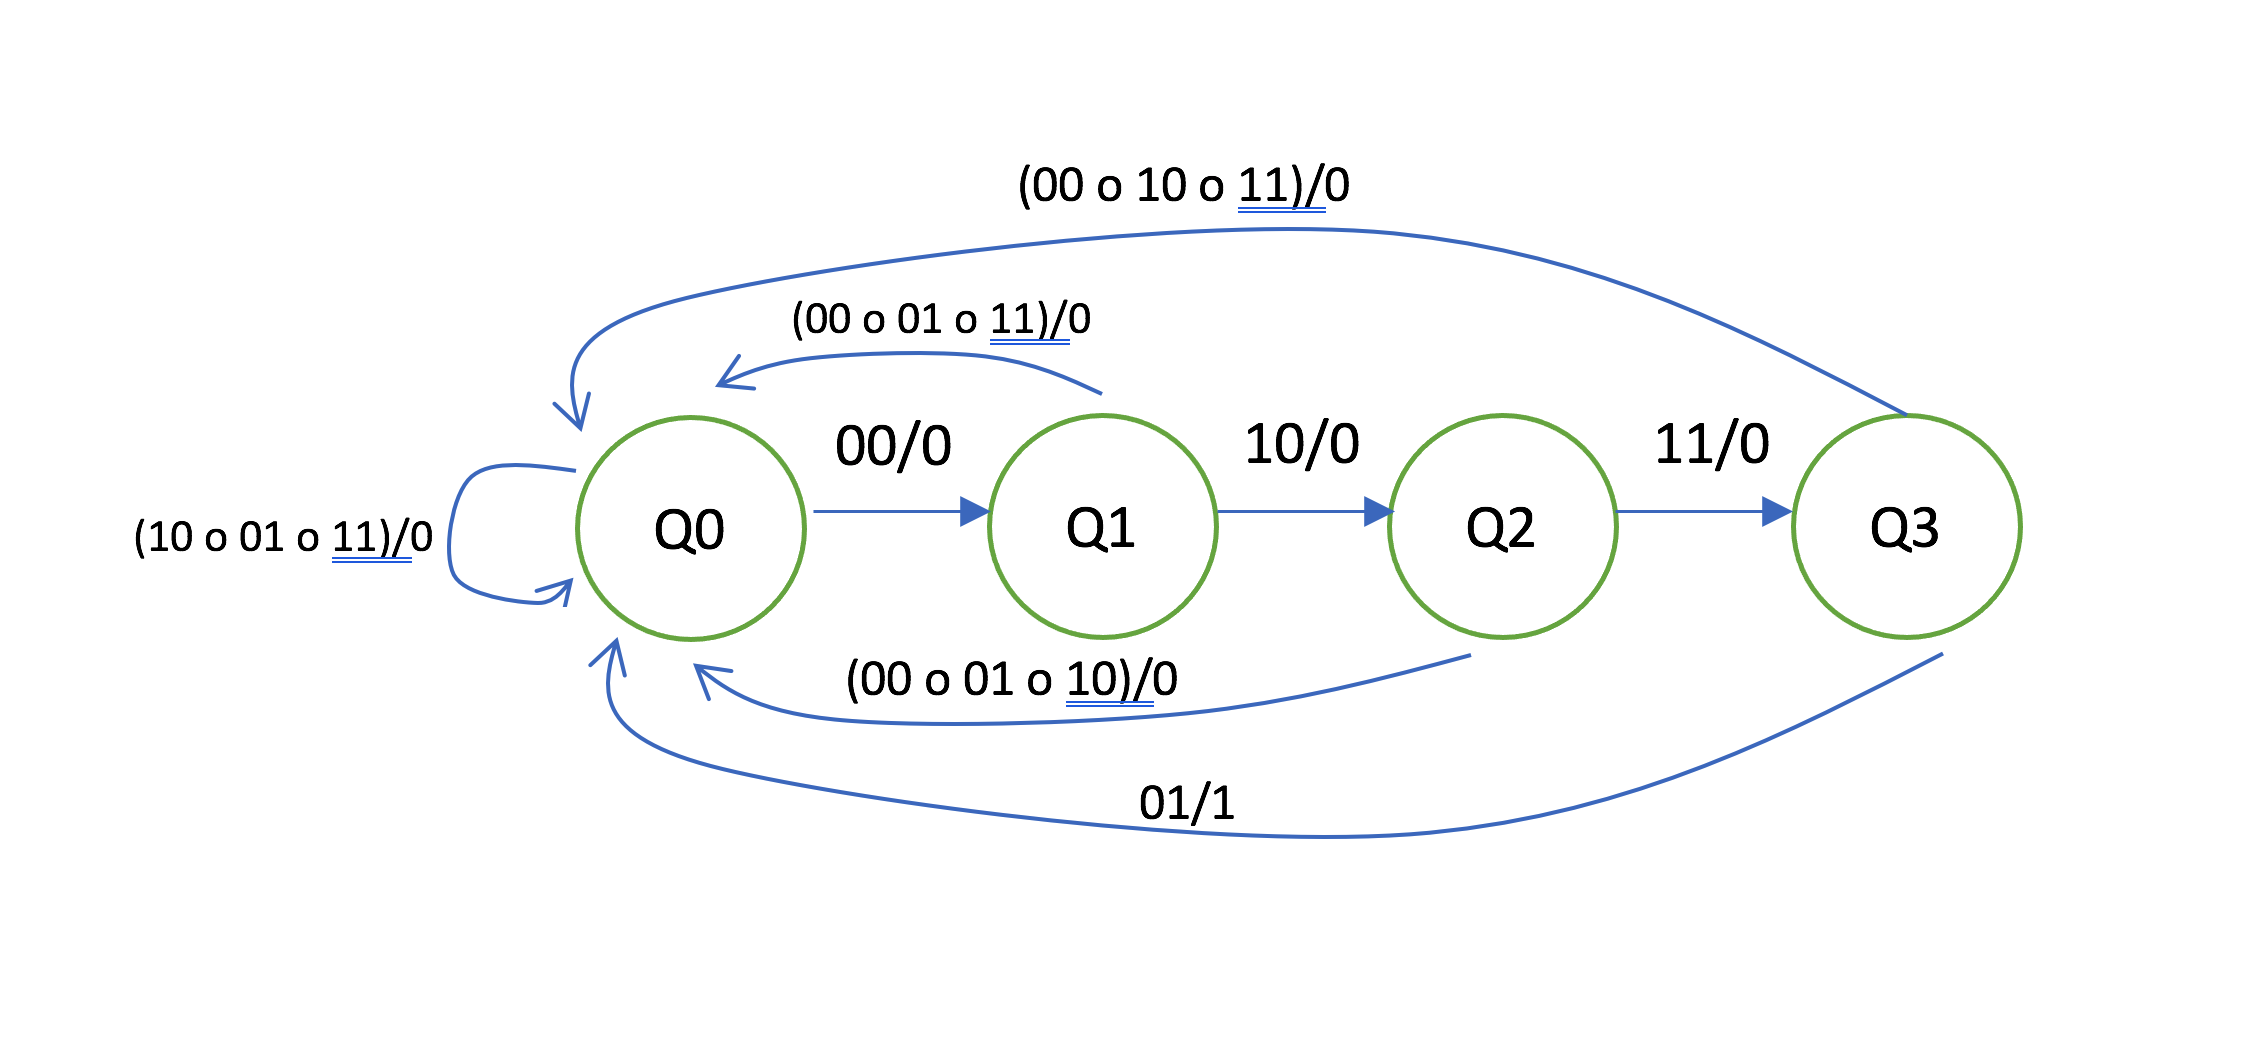
\includegraphics[width=130mm]{ApartatA.png}
		\end{center}
	\end{figure}
	
	\textbf{b)}  A partir del diagrama anterior crearem una taula d'estats. En primer lloc assignarem valors als estats.
	
	\begin{table}[h!]
		\centering
		 \begin{tabular}{|c | c|} 
			 \hline
			  Q0 &  00\\ 
			  \hline
			  Q1 &  01\\ 
			 \hline
			 Q2 & 10\\ [0.5ex] 
			 \hline
			 Q3 & 11\\ 
			 \hline
		 \end{tabular}
	\end{table}
	
	Ara creem la taula d'estats on Q es l'estat on es troba, $Q^+$ es l'estat on va a parar amb l'entrada corresponent, z es la sortida del sistema, $J_1$, $K_1$, $J_0$ i $K_0$ les entrades dels biestables.
	
	\begin{table}[h!]
		\centering
		 \begin{tabular}{| c | c | c | c | c | c | c | c |} 
		 	 \hline
			 Entrada & Q & $Q^+$ & z & $J_1$ & $K_1$ & $J_0$ & $K_0$\\
			 \hline\hline
			  00 &  00 & 01 & 0 & 0 & x & 1 & x\\ 
			  \hline
			  01/10/11 &  00 & 00 & 0 & 0 & x & 0 & x\\ 
			 \hline
			 10 &  01 & 10 & 0 & 1 & x & x & 1\\ 
			  \hline
			  00/01/11 &  01 & 00 & 0 & 0 & x & x & 1\\ 
			  \hline
			 11 &  10 & 11 & 0 & x & 0 & 1 & x\\ 
			  \hline
			  00/01/11 &  10 & 00 & 0 & x & 1 & 0 & x\\ 
			  \hline
			 01 &  11 & 00 & 1 & x & 1 & x & 1\\ 
			  \hline
			  00/10/11 &  11 & 00 & 0 & x & 1 & x & 1\\ 
			 \hline
		 \end{tabular}
	\end{table}
	
	Per tant ara podem concluir rapidament que podem simplificar rapid $K_0 = 1$. Per altra banda, si anomenem $e_1$ i $e_0$ el primer i segon bit de la entrada respectivament i $Q_1$ i $Q_0$ el primer i segon bit del estat, es pot simplificar $z = \overline{e_1}e_0Q_1Q_0$.
	
	Apliquem taules de Karnaugh per a simplificar els altres resultats a on les files seran els valors constants de $e_1$ i $e_0$ i les columnes els valors constants de $Q_1$ i $Q_0$
	
	En primer lloc busquem el valor simplificat de $J_1$.
	
	\begin{table}[!h]
		\centering
		\begin{tabular}{| c | c | c | c | c |}
			\hline
				&00	&01	&11	&10	\\
			\hline
			00	&0	&0	&X	&X	\\
			\hline
			01	&0	&0	&X	&X	\\
			\hline
			11	&0	&0	&X	&X	\\
			\hline
			10	&0	&1	&X	&X	\\
			\hline
		\end{tabular}
	\end{table}
	
	Podem fer un grup de 2 uns i per tant $J_1 = e_1\overline{e_0}Q_0$.
	
	Ara busquem el valor simplificat de $K_1$
	
	\begin{table}[!h]
		\centering
		\begin{tabular}{| c | c | c | c | c |}
			\hline
				&00	&01	&11	&10	\\
			\hline
			00	&X	&X	&1	&1	\\
			\hline
			01	&X	&X	&1	&1	\\
			\hline
			11	&X	&X	&1	&0	\\
			\hline
			10	&X	&X	&1	&1	\\
			\hline
		\end{tabular}
	\end{table}
	
	En aquest cas fem un grup de 2 zeros i obtenim $K_1 = \overline{e_1} + \overline{e_0} + Q_0$
	
	Finalment busquem el valor de $J_0$.
	
	\begin{table}[!h]
		\centering
		\begin{tabular}{| c | c | c | c | c |}
			\hline
				&00	&01	&11	&10	\\
			\hline
			00	&1	&X	&X	&0	\\
			\hline
			01	&0	&X	&X	&0	\\
			\hline
			11	&0	&X	&X	&1	\\
			\hline
			10	&0	&X	&X	&0	\\
			\hline
		\end{tabular}
	\end{table}
	
	Per a aquest cas fem dos grups de dos uns i obtenim $J_0 =  \bar{e_1}\bar{e_0}\overline{Q_1} + e_1e_0Q_1$
	
	Ara doncs ja podem dibuixar la estructura del circuit amb nomes 2 biestables.
	
	\begin{figure}[H]
		\begin{center}
		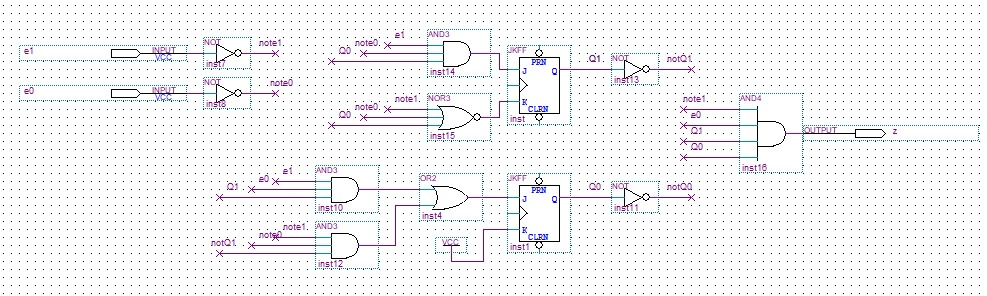
\includegraphics[width=140mm]{DisenyB.jpeg}
		\end{center}
	\end{figure}
	
	\textbf{c)}
	
	\begin{figure}[H]
		\begin{center}
		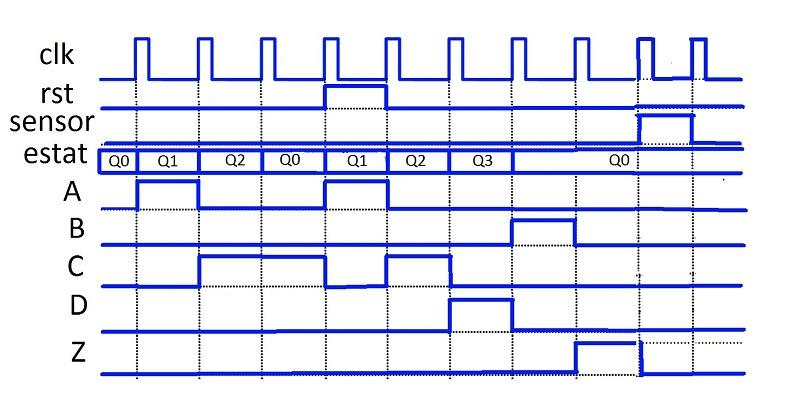
\includegraphics[width=130mm]{cronogramaBo.jpeg}
		\end{center}
	\end{figure}
	
	\textbf{d)} Una possible implementació del component requerit seria la següent.
	
	\begin{lstlisting}[style=vhdl, frame=single, basicstyle=\small]
library ieee;
use ieee.std_logic_1164.all;

entity led_porta is
    port( act : in std_logic;  
        leds : out std_logic_vector(7 down to 0)); %Error
end led_porta;

architecture arc of led_porta is %Error
type machine is ( st_obert , st_tancat );
signal le : std_logic_vector(7 down to 0) ;  
signal state : machine;
begin
   process(clk , nrst)
   begin
       case state is
            when st_obert => leds <= "11111111";
            when st_tancat  => leds <="00000000" ;
       end case;
   end process;
   leds <= le;
end arc;
	\end{lstlisting}
\end{document}



